\chapter{Numerical Results - Elastoplasticity} \label{chapter:numerical_results_elastoplasticity}

In the following chapter, results pertaining to elastoplasticity are presented.
The validation of the FFT-based Galerkin formulation is performed on elastoplastic materials at
small strains and large strains.
The constitutive model considered is the von Mises material model.

As in the previous chapter, all the numerical results shown in this chapter are obtained
in the same machine with the specifications provided in Table~\ref{tab:specifications}.
Contrary to the previous chapter, all the available cores in the machine are used in each simulation.

\section{Material characterization}

The microstructures and linear elastic properties considered in the following can be found in Section~\ref{sec:microstructures}.
The isotropic piecewise linear strain hardening law is presented in Figure~\ref{fig:von_mises_res_mat_small_strain_2D_normal_hardening_curve}.
The yield stress, \(\sigma_y\), is given as a function of the accumulated plastic strain, \(\bar{\varepsilon}_p\) by
\begin{equation}
\label{von_mises_hardening_curve}
  \sigma_y = \begin{cases}
    0.5 + 5\bar{\varepsilon}_p,\quad 0 \leq \bar{\epsilon}_p \leq 0.04\\
    0.7 + 2(\bar{\varepsilon}_p-0.04),\quad \bar{\epsilon}_p \geq 0.04\\
  \end{cases},\quad\si{\mega\pascal}.
\end{equation}

\begin{figure}[hbtp]
  \centering
  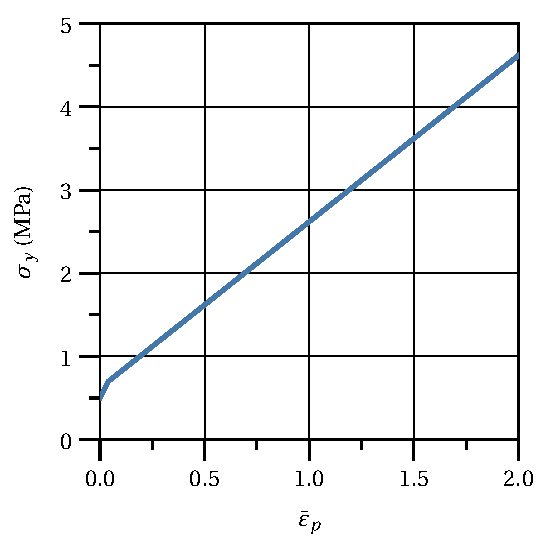
\includegraphics[width=0.5\textwidth]{figures/von_mises_res_mat_small_strain_2D_normal_hardening_curve}
  \caption{Von Mises elastoplastic matrix isotropic piecewise linear strain hardening law.}
\label{fig:von_mises_res_mat_small_strain_2D_normal_hardening_curve}
\end{figure}

\subsection{von Mises - small strains}

\paragraph{Constitutive model}
The model considered here for the elastoplastic behavior of the material is the von Mises model with associative potential and isotropic hardening, also known as standard \(J_{2}\)-plasticity.
In this model the total strain, \(\bm \varepsilon\), is additively split into an elastic part, \(\bm \varepsilon^e\), and a plastic part, \(\bm \varepsilon^p\), i.e.
\begin{equation}
\bm \varepsilon=\bm \varepsilon^e+\bm \varepsilon^p,
\end{equation}
The stress, \(\bm\sigma\), depends on the elastic strain, \(\bm \varepsilon^{e}\), through the standard linear relation
\begin{equation}
\bm \sigma=\boldsf{D}^{e}:\left(\bm \varepsilon-\bm\varepsilon^p\right), \quad \text { with } \quad \boldsf{D}^e \equiv 2 G \boldsf{I}_{S}+\left(K-\frac{2}{3} G\right) \boldsymbol{I} \otimes \boldsymbol{I},
\end{equation}
wherein \(K\) is the bulk modulus, \(G\) is the shear modulus and \(\boldsf I_d\).
The elastic domain is bounded by the plastic admissibility condition
\begin{equation}
\Phi\left(\bm \sigma, \bar{\varepsilon}^p\right) =\sigma_\text{eq} - \sigma_y(\bar{\varepsilon}^p)\leq 0,
\end{equation}
where \(\sigma_y\) is the hardening curve.
The deformation history enters this expression via the accumulated plastic strain, \(\bar{\varepsilon}^p\), which equals zero in the initial stress-free state.

Finally, the von Mises equivalent stress, \(\sigma_{\text {eq }}\), is defined as
\begin{equation}
\sigma_\text{eq}=\sqrt{\frac{3}{2} \bm s: \bm s},
\end{equation}
with \(\bm s\) the stress deviator.
The plastic strain rate follows from the associative potential or normality as
\begin{equation}
\dot{\varepsilon}^p=\dot{\gamma} \bm{N}=\dot{\gamma} \frac{\partial \Phi}{\partial \boldsymbol{\sigma}}=\dot{\gamma} \sqrt{\frac{3}{2}} \frac{\bm s}{\|\bm s\|}.
\end{equation}

The accumulated plastic strain is determined from
\begin{equation}
\bar{\varepsilon}^p=\int_{0}^{t} \dot{\varepsilon}^p \mathrm{d} t, \quad \text { with } \quad \dot{\varepsilon}^p=\sqrt{\frac{2}{3} \dot{\varepsilon}^p: \dot{\varepsilon}^p}=\dot{\gamma}
\end{equation}

The model is discretized in time using the, unconditionally stable, backward Euler scheme.
The stress update is implemented using an elastic-predictor plastic-corrector scheme, whereby the amount of plastic flow is determined in two steps.
First, a trial state is calculated by assuming the increment in strain to be fully elastic, the elastic predictor.
Second, if necessary, a return-map is used that quantifies the plastic strain increment, the plastic corrector.

Given an increment in total strain
\begin{equation}
\Delta \bm \varepsilon=\bm\varepsilon_{n+1}-\bm \varepsilon_n,
\end{equation}
corresponding to a typical pseudo-time increment \([t_n, t_{n+1}]\), the trial state, or elastic predictor, denoted by \((\bullet)^\text{trial}\), is computed by assuming that \(\Delta \bm \varepsilon\) gives rise to a purely elastic strain increment, i.e.,
\begin{align}
\bm \varepsilon_{n+1}^{e \text { trial }}&=\bm \varepsilon_{n}^{e}+\Delta \bm \varepsilon, \\
\bar{\varepsilon}_{n+1}^{p \text { trial }}&=\bar{\varepsilon}_{n}^{p}.
\end{align}
The corresponding trial stress is computed as
\begin{equation}
\sigma_{n+1}^{\text {trial }}=\boldsf{D}^{e}: \varepsilon_{n+1}^{e \text { trial }}.
\end{equation}

The trial yield stress is simply
\begin{equation}
\sigma_{y\:n+1}^{\text {trial }}=\sigma_{y}\left(\bar{\varepsilon}_{n}^{p}\right)={\sigma_{y}}_n,
\end{equation}
Having computed the elastic trial state, the next step in the algorithm is to check whether \(\sigma_{n+1}^{\text {trial }}\) lies inside or outside of the trial yield surface.
If \(\bm \sigma_{n+1}^{\text {trial }}\) lies inside of the trial yield surface, i.e. if
\begin{equation}
\Phi\left(\bm \sigma_{n+1}^{\text {trial }},\bar{\varepsilon}_{n+1}^{p \text { trial }} \right) \leq 0,
\end{equation}
then the process within the interval \(\left[t_{n}, t_{n+1}\right]\) is purely elastic and the elastic trial state itself is the solution to the integration problem. In this case,
\begin{align}
\bm\varepsilon_{n+1}^{e}&=\bm\varepsilon_{n+1}^{e \text { trial }}, \\
\bm\sigma_{n+1}&=\bm\sigma_{n+1}^{\text {trial }}, \\
\bar{\varepsilon}_{n+1}^{p}&=\bar{\varepsilon}_{n+1}^{p \text { trial }}=\bar{\varepsilon}_{n}^{p}, \\
\sigma_{y\:n+1}&=\sigma_{y\:n+1}^{\text {trial }}={\sigma_{y}}_n.
\end{align}

Otherwise, the process is elastoplastic within the interval \(\left[t_{n}, t_{n+1}\right]\) and the return mapping procedure has to be applied to return the trial state to an admissible state.
For this state, the equality needs to hold in the yield function, given the actual stress that in turn depends on the plastic flow.
Due to the assumed associative potential or normality, this non-linear system of equations can be rewritten as a single scalar equation
\begin{equation}
\bar{\Phi}(\Delta \gamma)= \sigma_{\text{eq}\:n}^\text{trial}-3 G \Delta \gamma-\sigma_y(\bar{\epsilon}_n^p+\Delta \gamma)=0,
\end{equation}
which has to be solved for \(\Delta \gamma\).

The resulting state can is then determined as
\begin{align}
\bm\varepsilon^p_{n+1}&=\bm\varepsilon^p_n+\Delta \gamma \bm{N}^\text{trial}, \\
\bar{\varepsilon}^p_{n+1}&=\bar{\varepsilon}^p_n+\Delta \gamma,\\
\bm\sigma_{n+1}&=\boldsf D^e:\left(\bm\varepsilon_{n+1}-\bm\varepsilon^p_ {n+1}\right).
\end{align}



\paragraph{Consistent constitutive tangent}
The tangent is derived by linearizing the stress update procedure.
If the trial state is elastic, i.e. when \(\Phi^\text{trial} \leq 0\), the result is trivially \(\boldsf{D}=\boldsf{D}^e\).
Otherwise, the stress update needs to be linearized, giving
\begin{equation}
\begin{aligned}
\boldsf D^\text{ep} &=\frac{\partial \bm{\sigma}_ {n+1}}{\partial \bm \varepsilon_ {n+1}} \\
&=\boldsf D^e-\frac{6 G^{2} \Delta \gamma}{\sigma_{\mathrm{eq}\:n}^\text{trial}} \boldsf{I}_{\mathrm{d}}+4 G^{2}\left(\frac{\Delta \gamma}{\sigma_{\mathrm{eq}\:n}^\text{trial}}-\frac{1}{3 G+ \displaystyle{\frac{\partial \sigma_y}{\partial \bar{\varepsilon}^p}}(\bar{\epsilon}_p+\Delta \gamma)}\right)\bm N^\text{trial} \otimes\bm N^\text{trial}.
\end{aligned}
\end{equation}

\subsection{von Mises - large strains}

The extension of the von Mises constitutive model from the context of small strains to large strains rests solely on a pre and post-processing step.
The remaining procedure regarding the state update and the consistent constitutive tangent is the same.

\paragraph{Pre-processing}

To enforce a multiplicative split of the elastic and plastic parts of the deformation gradient, the strain measure used instead of the small strain tensor is the Eulerian logarithmic strain tensor
\begin{equation}
  \bm \varepsilon \equiv \ln \bm V = \frac{1}{2}\ln \bm B,
\end{equation}
where \(\bm B = \bm F\bm F^T\) is left Cauchy-Green strain tensor, and \(\bm F\) the deformation gradient.

\paragraph{Post-processing}

The post-processing concerns the state update and the consistent tangent.
For the state update, the first Piola-Kirchhoff stress tensor can be obtained as
\begin{equation}
\bm P = \bm \tau \bm F^{-T},
\end{equation}
keeping in mind that the stress measure output having used the pre-processing is the Kirchhof stress tensor \(\bm \tau\).

Regarding the spatial consistent tangent, it is obtained using the expression in Equation~\eqref{eq:space_consistent_tangent}, with the only difference being that instead of the elasticity tensor \(\boldsf D^e\) the elastoplastic tensor \(\boldsf D^\text{ep}\) is used.

\section{Comparison between FFT and FEM-based homogenization}

\paragraph{Small strain}

Only the two-dimensional microstructure described in Section~\ref{sec:microstructures} is again considered together with the elastic properties described in Table~\ref{tab:mat_properties}.
Due to time constraints results for the three-dimensional microstructure are not included.
The matrix is now assumed elastoplastic with a von Mises associative flow rule and the isotropic piecewise linear strain hardening law illustrated in Figure~\ref{fig:von_mises_res_mat_small_strain_2D_normal_hardening_curve}.
Only small strains are considered.
Periodic boundary conditions are adopted and the following two macroscale strain loading cases are considered
\begin{equation}
\text { uniaxial: } \bm{\varepsilon}=\left[\begin{array}{cc}
5 & 0 \\
0 & 0
\end{array}\right] \times 10^{-2}, \quad \text { pure shear: } \quad \bm \varepsilon=\left[\begin{array}{cc}
0 & 2.5 \\
2.5 & 0
\end{array}\right] \times 10^{-2},
\end{equation}
being enforced in a total of 200 increments.
Note that in the 2D plane strain case, only the in-plane \(O_{x y}\) macroscale strain components are enforced.
In terms of spatial discretization, a grid \(n_{v}=600 \times 600\) is considered.
The convergence criterion used is Criterion II, as described in Section~\ref{sec:criteria}.

The homogenized response of the fiber-reinforced composite under uniaxial and pure shear strain loading conditions is presented in Figures~\ref{fig:von_mises_res_mat_small_strain_2D_normal_material_response_and_error} and \ref{fig:von_mises_res_mat_small_strain_2D_shear_material_response_and_error}.
The relative error with respect to the FEM reference solution is also shown.
An excellent agreement between the two solutions is found.
Moreover, the error is below 0.15\% for the whole deformation history.
The local strain fields can be found in Figure \ref{fig:von_mises_res_mat_small_strain_2D_normal_local_fields} and \ref{fig:von_mises_res_mat_small_strain_2D_shear_local_fields}.
Again, visually there is no detectable difference between the local field computed using the two different approaches.

In terms of computational performance, Table~\ref{tab:von_mises_small_strain_2D_cpu_time} shows that the FTT approach is around 20 times faster than the FEM approach.
It is difficult to tell if this time difference is due to the greater efficiency of the FFT approach or a larger amount of pre and post-processing steps used in the FEM implementation used.
See Section~\ref{sec:hencky_accuracy_validation} for an example of the impact of pre and post-processing operation during state update in the execution time of the FFT approach.

From these results, it follows regarding the application of the FFT-Gakerin method to an elastoplastic material that:
\begin{itemize}
  \item At small strains, the homogenized response is accurate and the error, when compared with the FEM solution, is very small (\(<0.15\%\));
  \item The local fields are also in agreement with the FEM solution.
  \item Regarding efficiency, the FTT-Galerkin method is 20 times faster than the FEM method for both loading schemes considered.
\end{itemize}

\begin{table}[htbp]
  \caption{Comparison between the CPU time required by the FFT-based and FEM-based homogenization approaches in the
  solution of the fiber-reinforced (fibers: linear elastic; matrix: elastoplastic with a von Mises associative flow rule and the isotropic piecewise linear strain hardening law) composite equilibrium problem under uniaxial and pure
  strain loading conditions (\(n_v = 600 \times 600\)).}
\label{tab:von_mises_small_strain_2D_cpu_time}
  \centering
    \begin{tabular}{
       c
       S[
       scientific-notation = true,
         table-format=1.2e-2,
                   round-mode=places,
         round-precision=2
         ]
       S[
       scientific-notation = true,
         table-format=1.2e-2,
                   round-mode=places,
         round-precision=2
         ]
      }
    & \multicolumn{2}{c}{CPU Time (s)} \\ \cline{2-3}
    \vphantom{\Big |}Loading scheme & {FFT} & {FEM} \\
    \hline\hline
    \vphantom{\Big |}Uniaxial strain & 1.24e+03 & 0.1996E+05 \\
    Pure shear strain & 2.87e+03 & 0.3636E+05  \\
    \hline\hline
  \end{tabular}
\end{table}

\begin{figure}[hbt]
  \centering
  	\begin{subfigure}[b]{0.49\textwidth}
      \centering
      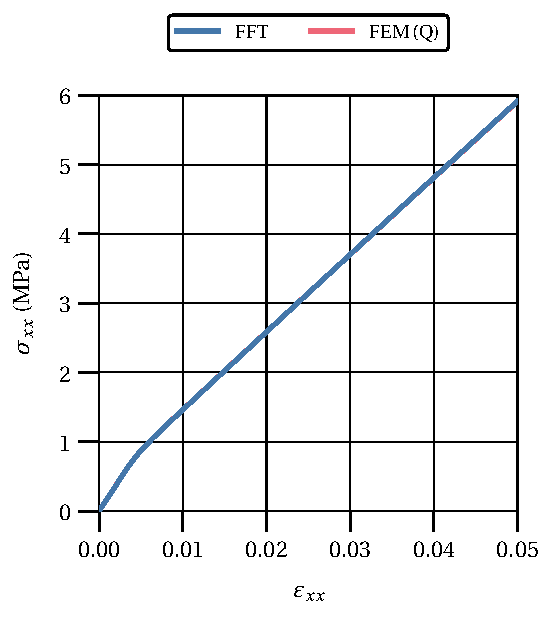
\includegraphics[width=\textwidth]{figures/von_mises_res_mat_small_strain_2D_normal_material_response}
      \caption{}
      \label{subfig:von_mises_res_mat_small_strain_2D_normal_material_response}
    \end{subfigure}
    \begin{subfigure}[b]{0.49\textwidth}
      \centering
      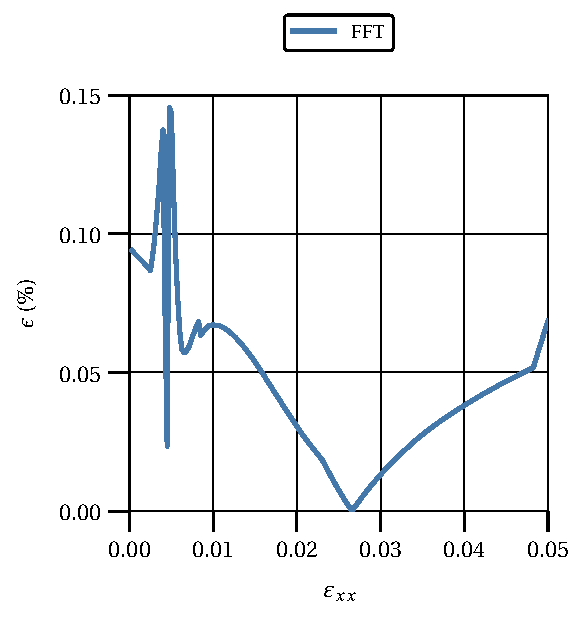
\includegraphics[width=\textwidth]{figures/von_mises_res_mat_small_strain_2D_normal_material_response_error}
      \caption{}
      \label{subfig:von_mises_res_mat_small_strain_2D_normal_material_response_error}
    \end{subfigure}
  \caption{Comparison between the FFT and FEM-based homogenization approaches in the solution
  of the fiber-reinforced (fibers: linear elastic; matrix: elastoplastic with a von Mises associative flow rule and the isotropic piecewise linear strain hardening law) composite equilibrium problem under normal strain
  loading conditions: \subref{subfig:von_mises_res_mat_small_strain_2D_normal_material_response} Homogenized
  stress; \subref{subfig:linear_2D_normal_stress_avg_cpu_time_vs_n_voxels} Relative error of the homogenized material response obtained with the FFT approach relative to the FEM approach;
  Notation: quadratic element (Q).}
\label{fig:von_mises_res_mat_small_strain_2D_normal_material_response_and_error}
\end{figure}

\begin{figure}[hbt]
  \centering
	\begin{subfigure}[b]{\textwidth}
    \centering
    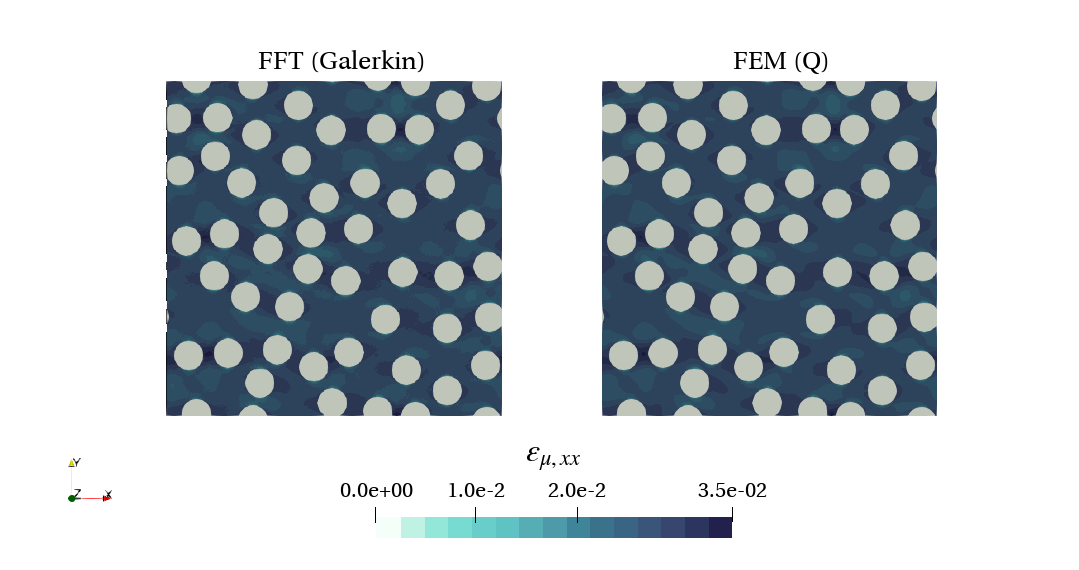
\includegraphics[width=\textwidth]{figures/von_mises_res_mat_small_strain_2D_normal_elastic_strain_11}
    \caption{}
    \label{subfig:von_mises_res_mat_small_strain_2D_normal_elastic_strain_11}
  \end{subfigure}
  \begin{subfigure}[b]{\textwidth}
    \centering
    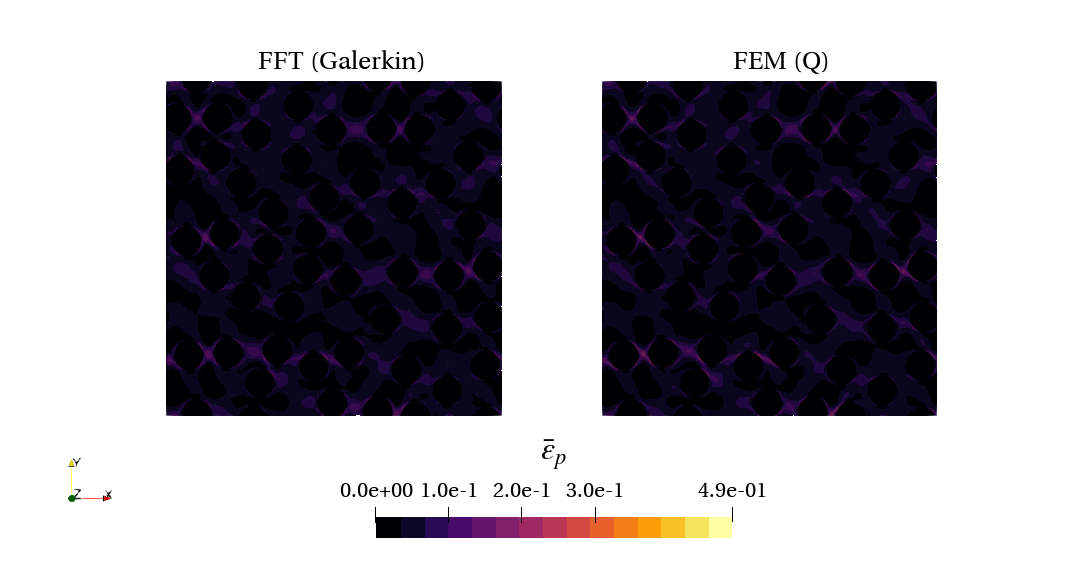
\includegraphics[width=\textwidth]{figures/von_mises_res_mat_small_strain_2D_normal_palstic_strain_11}
    \caption{}
    \label{subfig:von_mises_res_mat_small_strain_2D_normal_palstic_strain_11}
  \end{subfigure}
  \caption{Comparison between the FFT-based and FEM-based homogenization approaches in the
  solution of the fiber-reinforced (fibers: linear elastic; matrix: elastoplastic with a von Mises associative flow rule and the isotropic piecewise linear strain hardening law) composite equilibrium problem under uniaxial
  strain loading conditions: \subref{subfig:von_mises_res_mat_small_strain_2D_normal_elastic_strain_11} Local elastic strain field, \(\varepsilon_{\mu,xx}\), of the matrix phase at full load; \subref{subfig:von_mises_res_mat_small_strain_2D_normal_palstic_strain_11} Local accumulated plastic strain field, \(\bar{\varepsilon}_{p}\), of the matrix phase at full load.  (\(n_v = 600 \times 600\) discretization). Notation: quadratic element (Q).}
\label{fig:von_mises_res_mat_small_strain_2D_normal_local_fields}
\end{figure}

\begin{figure}[hbt]
  \centering
  	\begin{subfigure}[b]{0.49\textwidth}
      \centering
      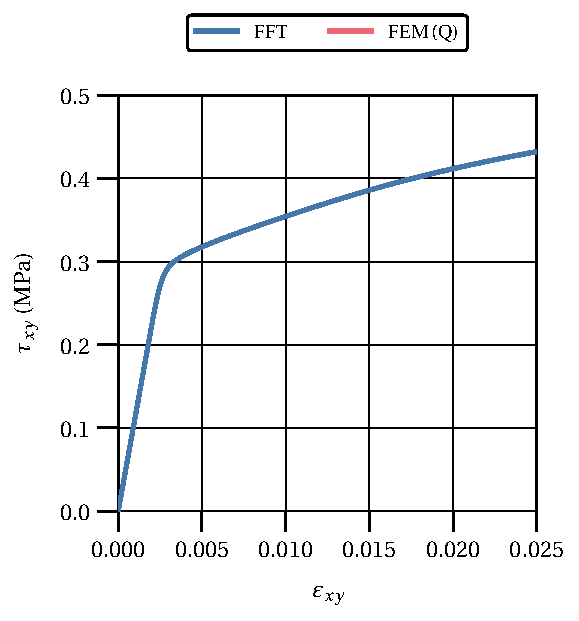
\includegraphics[width=\textwidth]{figures/von_mises_res_mat_small_strain_2D_shear_material_response}
      \caption{}
      \label{subfig:von_mises_res_mat_small_strain_2D_shear_material_response}
    \end{subfigure}
    \begin{subfigure}[b]{0.49\textwidth}
      \centering
      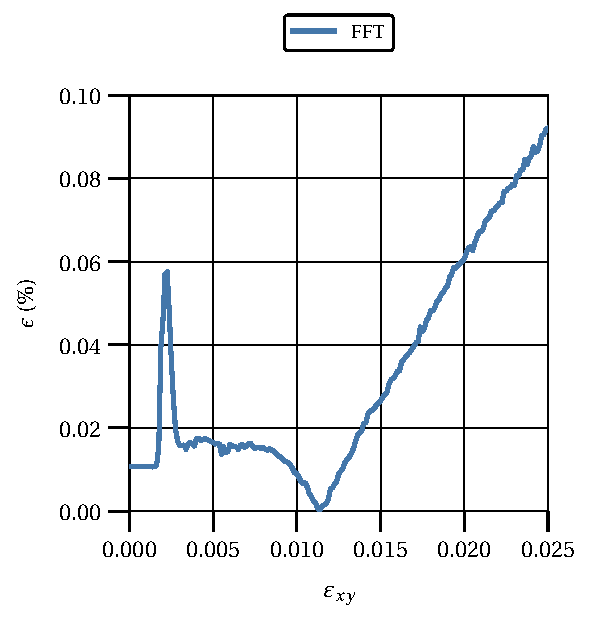
\includegraphics[width=\textwidth]{figures/von_mises_res_mat_small_strain_2D_shear_material_response_error}
      \caption{}
      \label{subfig:von_mises_res_mat_small_strain_2D_shear_material_response_error}
    \end{subfigure}
  \caption{Comparison between the FFT and FEM-based homogenization approaches in the solution
  of the fiber-reinforced (fibers: linear elastic; matrix: elastoplastic with a von Mises associative flow rule and the isotropic piecewise linear strain hardening law) composite equilibrium problem under normal strain
  loading conditions: \subref{subfig:von_mises_res_mat_small_strain_2D_shear_material_response} Homogenized
  stress; \subref{subfig:von_mises_res_mat_small_strain_2D_shear_material_response_error} Relative error of the homogenized material response obtained with the FFT approach relative to the FEM approach;
  Notation: linear element (L), quadratic element (Q).}
\label{fig:von_mises_res_mat_small_strain_2D_shear_material_response_and_error}
\end{figure}

\begin{figure}[hbt]
  \centering
	\begin{subfigure}[b]{\textwidth}
    \centering
    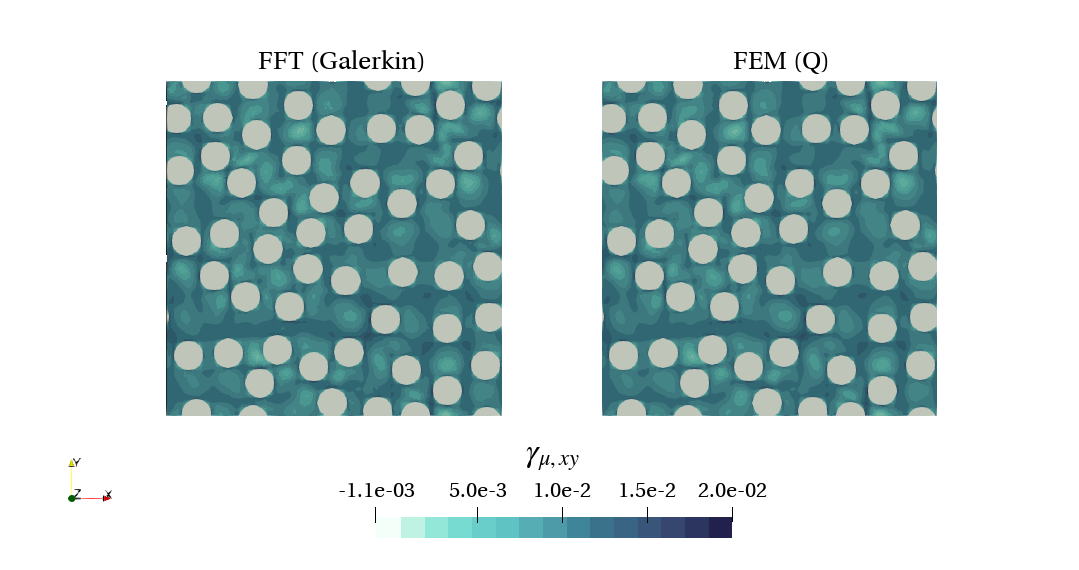
\includegraphics[width=\textwidth]{figures/von_mises_res_mat_small_strain_2D_shear_elastic_strain_12}
    \caption{}
    \label{subfig:von_mises_res_mat_small_strain_2D_shear_elastic_strain_12}
  \end{subfigure}
  \begin{subfigure}[b]{\textwidth}
    \centering
    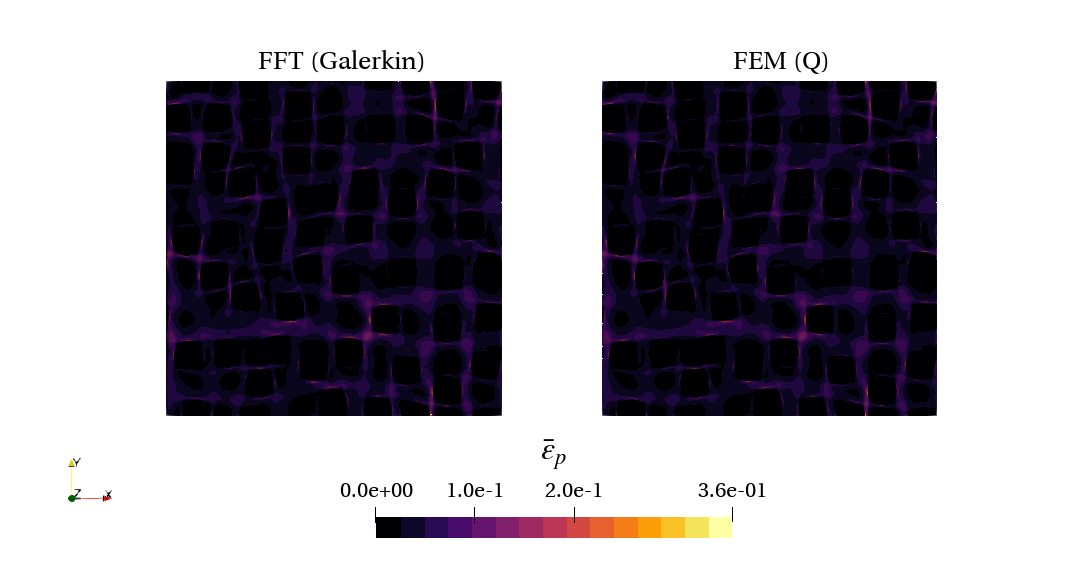
\includegraphics[width=\textwidth]{figures/von_mises_res_mat_small_strain_2D_shear_palstic_strain}
    \caption{}
    \label{subfig:von_mises_res_mat_small_strain_2D_shear_palstic_strain}
  \end{subfigure}
  \caption{Comparison between the FFT-based and FEM-based homogenization approaches in the
  solution of the fiber-reinforced (fibers: linear elastic; matrix: elastoplastic with a von Mises associative flow rule and the isotropic piecewise linear strain hardening law) composite equilibrium problem under uniaxial
  strain loading conditions: \subref{subfig:von_mises_res_mat_small_strain_2D_shear_elastic_strain_12} Local elastic strain field, \(\gamma_{\mu,xy}\), of the matrix phase at full load; \subref{subfig:von_mises_res_mat_small_strain_2D_shear_palstic_strain} Local accumulated plastic strain field, \(\bar{\varepsilon}_{p}\), of the matrix phase at full load.  (\(n_v = 600 \times 600\) discretization). Notation: quadratic element (Q).}
\label{fig:von_mises_res_mat_small_strain_2D_shear_local_fields}
\end{figure}



\FloatBarrier

\paragraph{Large strain}

Only the two-dimensional microstructure described in Section~\ref{sec:microstructures} is again considered together with the elastic properties described in Table~\ref{tab:mat_properties}.
The matrix is again assumed elastoplastic with a von Mises associative flow rule and the isotropic piecewise linear strain hardening law illustrated in Figure~\ref{fig:von_mises_res_mat_small_strain_2D_normal_hardening_curve}.
Large strains are considered.
Periodic boundary conditions are adopted and the following two macroscale strain loading cases are considered
\begin{equation}
\text { uniaxial: } \bm{F}=\left[\begin{array}{cc}
1.1 & 0.0 \\
0.0 & 1.0
\end{array}\right], \quad \text { pure shear: } \quad \bm F=\left[\begin{array}{cc}
1.0 & 0.3 \\
0.0 & 1.0
\end{array}\right],
\end{equation}
being enforced in a total of 200 increments.
Note that in the 2D plane strain case, only the in-plane \(O_{x y}\) macroscale strain components are enforced.
In terms of spatial discretization, a grid \(n_{v}=600 \times 600\) is considered.
The convergence criterion used is Criterion II, as described in Section~\ref{sec:criteria}.

The homogenized response of the fiber-reinforced composite under uniaxial and pure shear strain loading conditions is presented in Figures~\ref{fig:von_mises_res_mat_large_strain_2D_normal_material_response_and_error} and \ref{fig:von_mises_res_mat_large_strain_2D_shear_material_response_and_error}.
The relative error with respect to the FEM reference solution is also shown.
An excellent agreement between the two solutions is found for uniaxial strain loading.
Moreover, the error is below 0.1\% for the whole deformation history.
On the other hand, for the pure shear loading scheme the FFT-based approach fails to converge after \(F_{xy}=0.1\).
Immediately before the error starts to increase exponentially reaching around 1.6\%.

The local strain fields can be found in Figure \ref{fig:von_mises_res_mat_large_strain_2D_normal_local_fields} and \ref{fig:von_mises_res_mat_large_strain_2D_shear_local_fields}.
Again, visually there is no detectable difference between the local field computed using the two different approaches for the uniaxial strain loading scheme.
For the FFT-based approach, the local fields are not available at full load.
However, it can be gathered from the maximum values of the accumulated plastic strain, shown in Figure~\ref{subfig:von_mises_res_mat_large_strain_2D_shear_palstic_strain}, that it reaches values as a high as 1.4.
It is substantially larger than the maximum value found for the uniaxial strain loading scheme, \(\bar{\varepsilon}_p\approx 0.7\), thus making the particular pure shear strain loading scheme here considered more demanding.
This helps explain why only the uniaxial strain loading scheme reached full load.

In terms of computational performance, Table~\ref{tab:von_mises_large_strain_2D_cpu_time} shows that the FTT approach is around 1.5 times faster than the FEM approach for the uniaxial strain loading scheme.
However, as already mentioned, it fails to reach full load for the pure shear strain loading scheme.

From these results, it follows regarding the application of the FFT-Gakerin method to an elastoplastic material at large strains that:
\begin{itemize}
  \item The homogenized response is accurate and the error, when compared with the FEM solution, is very small (\(<0.15\%\)) for the more conservative uniaxial strain loading scheme prescribed.
  The local fields are also in agreement with the FEM solution and the FTT-Galerkin method is 1.5 times faster than the FEM method.
  \item For the more demanding pure shear loading scheme, the FFT-Galerkin method was not able to apply the full load.
  However, the homogenized response before failure is moderately accurate with errors relative to the FEM solution below \(1.6\%\).
\end{itemize}

\begin{table}[htbp]
  \caption{Comparison between the CPU time required by the FFT-based and FEM-based homogenization approaches in the
  solution of the fiber-reinforced (fibers: hyperelastic (Hencky constitutive model); matrix: elastoplastic with a von Mises associative flow rule and the isotropic piecewise linear strain hardening law) composite equilibrium problem under uniaxial and pure
  strain loading conditions (\(n_v = 600 \times 600\)).}
\label{tab:von_mises_large_strain_2D_cpu_time}
  \centering
    \begin{tabular}{
       c
       S[
       scientific-notation = true,
         table-format=1.2e-2,
                   round-mode=places,
         round-precision=2
         ]
       S[
       scientific-notation = true,
         table-format=1.2e-2,
                   round-mode=places,
         round-precision=2
         ]
      }
    & \multicolumn{2}{c}{CPU Time (s)} \\ \cline{2-3}
    \vphantom{\Big |}Loading scheme & {FFT} & {FEM} \\
    \hline\hline
    \vphantom{\Big |}Uniaxial strain & 16554.911 & 0.2357E+05 \\
    Pure shear strain & {-} & 0.6014E+05  \\
    \hline\hline
  \end{tabular}
\end{table}

\begin{figure}[hbt]
  \centering
  	\begin{subfigure}[b]{0.49\textwidth}
      \centering
      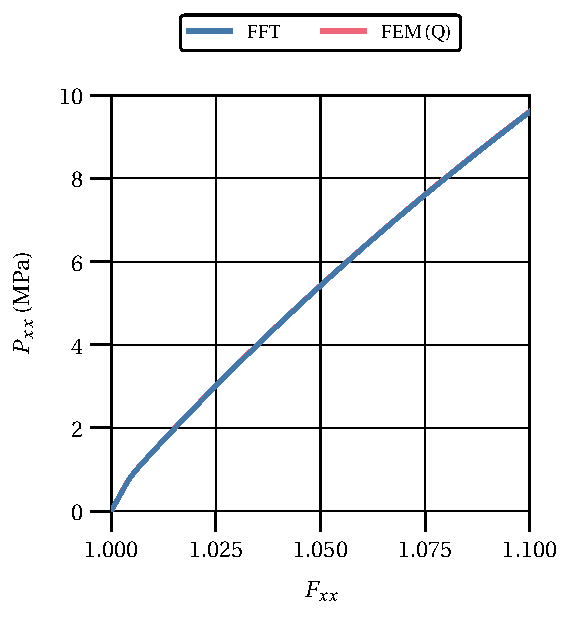
\includegraphics[width=\textwidth]{figures/von_mises_res_mat_large_strain_2D_normal_material_response}
      \caption{}
      \label{subfig:von_mises_res_mat_large_strain_2D_normal_material_response}
    \end{subfigure}
    \begin{subfigure}[b]{0.49\textwidth}
      \centering
      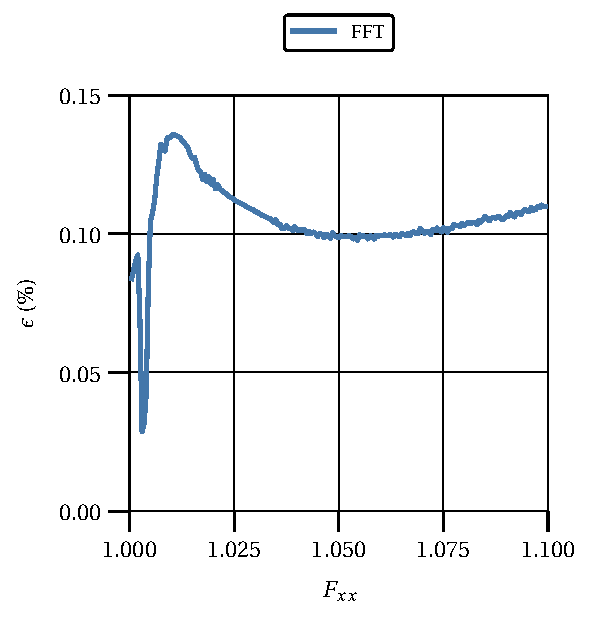
\includegraphics[width=\textwidth]{figures/von_mises_res_mat_large_strain_2D_normal_material_response_error}
      \caption{}
      \label{subfig:von_mises_res_mat_large_strain_2D_normal_material_response_error}
    \end{subfigure}
  \caption{Comparison between the FFT and FEM-based homogenization approaches in the solution of the fiber-reinforced (fibers: hyperelastic (Hencky constitutive model); matrix: elastoplastic with a von Mises associative flow rule and the isotropic piecewise linear strain hardening law) composite equilibrium problem under normal strain loading conditions: \subref{subfig:von_mises_res_mat_small_strain_2D_normal_material_response} Homogenized stress; \subref{subfig:linear_2D_normal_stress_avg_cpu_time_vs_n_voxels} Relative error of the homogenized material response obtained with the FFT approach relative to the FEM approach; Notation: quadratic element (Q).}
\label{fig:von_mises_res_mat_large_strain_2D_normal_material_response_and_error}
\end{figure}

\begin{figure}[hbt]
  \centering
	\begin{subfigure}[b]{\textwidth}
    \centering
    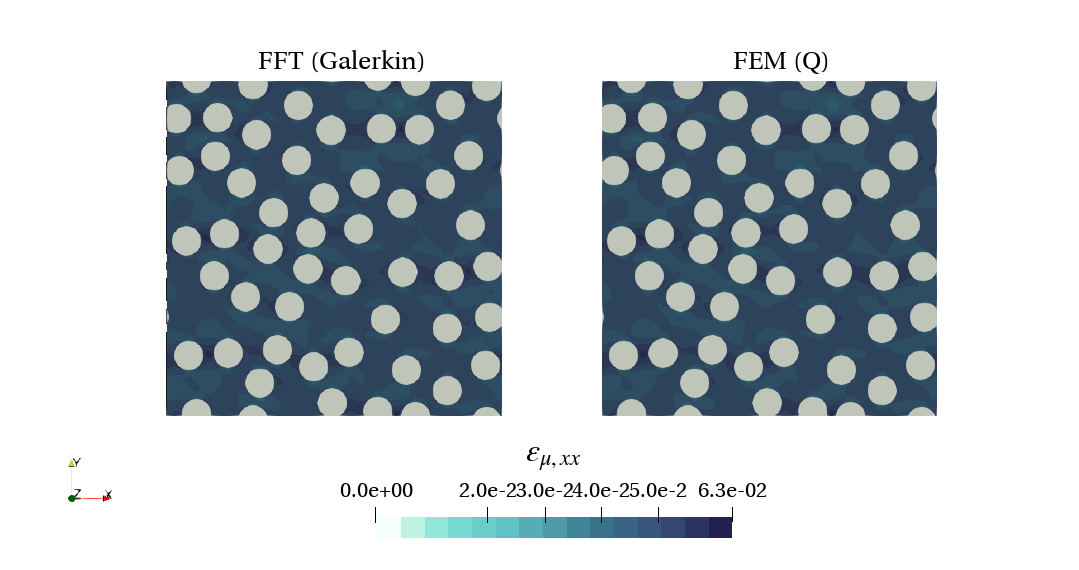
\includegraphics[width=\textwidth]{figures/von_mises_res_mat_large_strain_2D_normal_elastic_strain_11}
    \caption{}
    \label{subfig:von_mises_res_mat_large_strain_2D_normal_elastic_strain_11}
  \end{subfigure}
  \begin{subfigure}[b]{\textwidth}
    \centering
    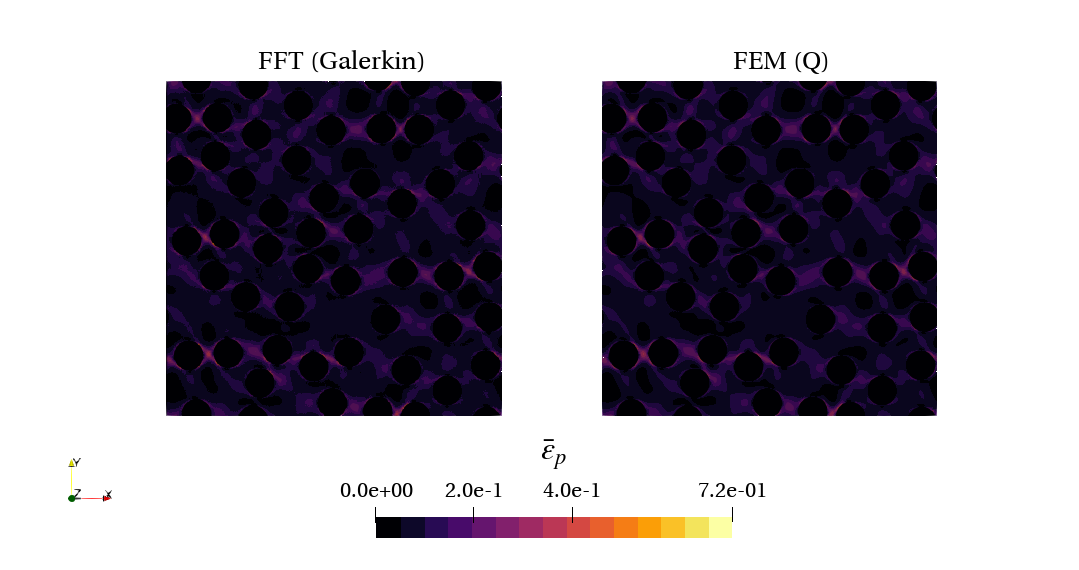
\includegraphics[width=\textwidth]{figures/von_mises_res_mat_large_strain_2D_normal_palstic_strain_11}
    \caption{}
    \label{subfig:von_mises_res_mat_large_strain_2D_normal_palstic_strain_11}
  \end{subfigure}
  \caption{Comparison between the FFT-based and FEM-based homogenization approaches in the
  solution of the fiber-reinforced (fibers: hyperelastic (Hencky constitutive model); matrix: elastoplastic with a von Mises associative flow rule and the isotropic piecewise linear strain hardening law) composite equilibrium problem under uniaxial
  strain loading conditions: \subref{subfig:von_mises_res_mat_large_strain_2D_normal_elastic_strain_11} Local elastic strain field, \(\varepsilon_{\mu,xx}\), of the matrix phase at full load; \subref{subfig:von_mises_res_mat_large_strain_2D_normal_palstic_strain_11} Local accumulated plastic strain field, \(\bar{\varepsilon}_{p}\), of the matrix phase at full load.  (\(n_v = 600 \times 600\) discretization). Notation: quadratic element (Q).}
\label{fig:von_mises_res_mat_large_strain_2D_normal_local_fields}
\end{figure}

\begin{figure}[hbt]
  \centering
  	\begin{subfigure}[b]{0.49\textwidth}
      \centering
      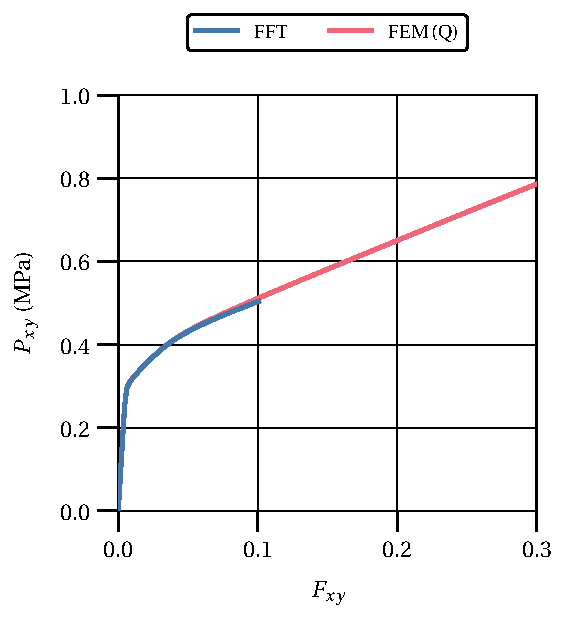
\includegraphics[width=\textwidth]{figures/von_mises_res_mat_large_strain_2D_shear_material_response}
      \caption{}
      \label{subfig:von_mises_res_mat_large_strain_2D_shear_material_response}
    \end{subfigure}
    \begin{subfigure}[b]{0.49\textwidth}
      \centering
      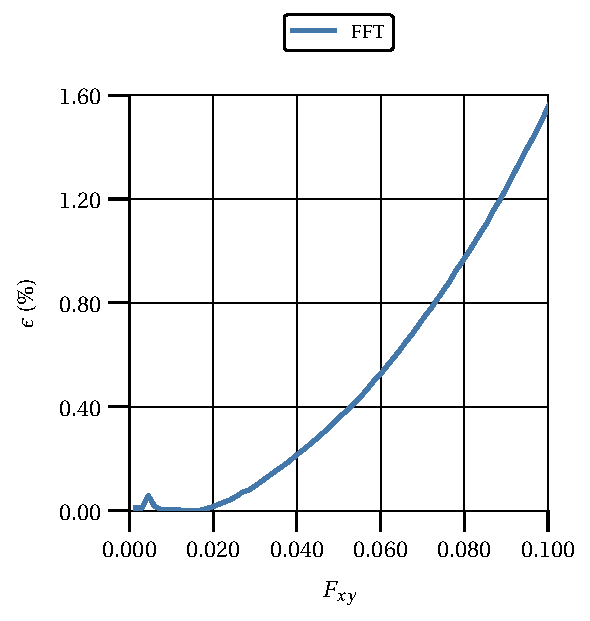
\includegraphics[width=\textwidth]{figures/von_mises_res_mat_large_strain_2D_shear_material_response_error}
      \caption{}
      \label{subfig:von_mises_res_mat_large_strain_2D_shear_material_response_error}
    \end{subfigure}
  \caption{Comparison between the FFT and FEM-based homogenization approaches in the solution of the fiber-reinforced (fibers: hyperelastic (Hencky constitutive model); matrix: elastoplastic with a von Mises associative flow rule and the isotropic piecewise linear strain hardening law) composite equilibrium problem under pure shear strain loading conditions: \subref{subfig:von_mises_res_mat_large_strain_2D_shear_material_response} Homogenized stress; \subref{subfig:von_mises_res_mat_large_strain_2D_shear_material_response_error} Relative error of the homogenized material response obtained with the FFT approach relative to the FEM approach; Notation: quadratic element (Q).}
\label{fig:von_mises_res_mat_large_strain_2D_shear_material_response_and_error}
\end{figure}

\begin{figure}[hbt]
  \centering
	\begin{subfigure}[b]{\textwidth}
    \centering
    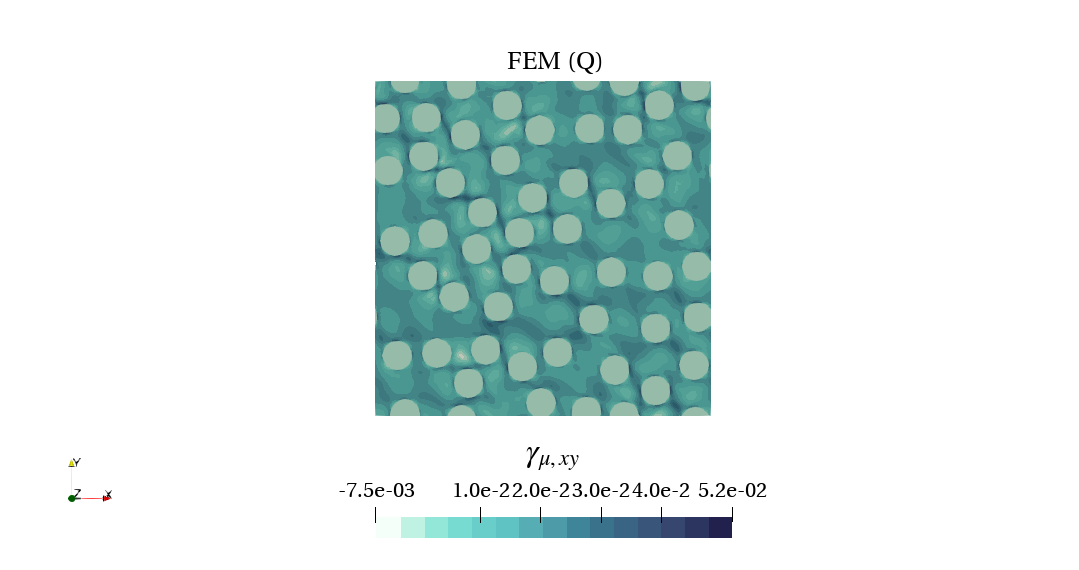
\includegraphics[width=\textwidth]{figures/von_mises_res_mat_large_strain_2D_shear_elastic_strain_12}
    \caption{}
    \label{subfig:von_mises_res_mat_large_strain_2D_shear_elastic_strain_12}
  \end{subfigure}
  \begin{subfigure}[b]{\textwidth}
    \centering
    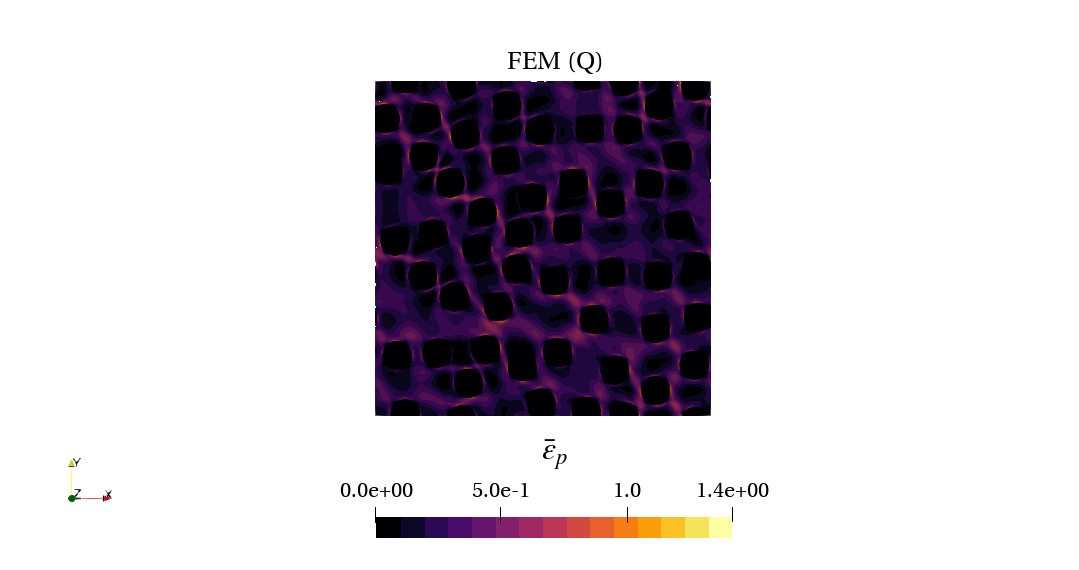
\includegraphics[width=\textwidth]{figures/von_mises_res_mat_large_strain_2D_shear_palstic_strain}
    \caption{}
    \label{subfig:von_mises_res_mat_large_strain_2D_shear_palstic_strain}
  \end{subfigure}
  \caption{Comparison between the FFT-based and FEM-based homogenization approaches in the
  solution of the fiber-reinforced (fibers: hyperelastic (Hencky constitutive model); matrix: elastoplastic with a von Mises associative flow rule and the isotropic piecewise linear strain hardening law) composite equilibrium problem under pure shear strain loading conditions: \subref{subfig:von_mises_res_mat_large_strain_2D_shear_elastic_strain_12} Local elastic strain field, \(\gamma_{\mu,xy}\), of the matrix phase at full load; \subref{subfig:von_mises_res_mat_large_strain_2D_shear_palstic_strain} Local accumulated plastic strain field, \(\bar{\varepsilon}_{p}\), of the matrix phase at full load  - Only FEM available since the FFT solution did not reach full load (\(n_v = 600 \times 600\) discretization). Notation: quadratic element (Q).}
\label{fig:von_mises_res_mat_large_strain_2D_shear_local_fields}
\end{figure}
